\chapter{Concepts and Technologies}\label{cha:concepts}
Throughout the development of this project quite a few tools and technologies were employed. To address them all, this chapter was broken in three sections; Front-end in Section~\ref{cha:concepts:sec:frontend}, that is focused mainly in user-facing web technologies; Back-end in Section~\ref{cha:concepts:sec:backend}, which is concerned with the developed Web \gls{API} and lastly; Development in Section~\ref{development}, with the tools used to write, build and test this project.

\section{Front-end}\label{cha:concepts:sec:frontend}
This section is concerned with the description of technologies used to assemble the human-interactive part of this project.


\subsection{Typescript}
`` A super-set of JavaScript that compiles to plain JavaScript ''~\cite{tswebsite}, Typescript is a language maintained by Microsoft and developed by \textit{Anders Hejlsberg} in 2012 with the goal of improving the quality and manageability of JavaScript code bases with features such as static typing and object-orientated qualities~\cite{tsrevealed}. Ultimately, Typescript must be compiled to JavaScript before being executed, for compatibility reasons, the default JavaScript target is version ES3 but newer back-ends are also available.

\subsection{HTML}
The \gls{HTML}, the `` World Wide Web's core markup language ''~\cite{html} is a declarative language through which the vast majority of online content is structured, shared and accessed. It is a specification of elements that can be used to structure the content of web pages, such as headings, images, link to other documents, buttons and many others~\cite{htmlcss}.

\subsection{CSS}
\gls{CSS} is another declarative language that pairs with HTML. Its purpose is to describe how the elements present in a web page are presented.
Some of definitions handle colors, fonts, element arranging, visibility, interaction and many others aspects~\cite{htmlcss}.

\subsection{SASS}
\gls{SASS} is a augmentation of CSS with features that are similar to a object-oriented languages, with loops, variables, functions and rule nesting ~\cite{sass}. SASS files need to be compiled into plain CSS before deployment, there are many of such compilers, some re-generate CSS files upon file  changes.

\subsection{Angular}\label{concept:angular}
Front-end web framework developed as a side project at Google that proved itself as a valuable tool for modern application development. The core idea is that \gls{HTML} faults when it comes to declare dynamic content~\cite{angularjs}, therefore a new middle-ware is introduced between the rendered page and the underling code so that all the elements and events in the \gls{HTML} document are captured and made available to its components. Such binding goes both ways, so if the state of the underling code changes, the document is re-rendered to reflect the new state.

The first version of Angular is now called AngularJs and can be included in a \gls{HTML} document just like any other JavaScript library. This version proved it's value but was considered confusing and some times, slow. Since then it entered \gls{LTS} stage and no features are added. Angular version 2 and up is a Typescript re-write that includes some new features that aid in the architecture and development of scalable and reusable code, namely, the introduction of Components, Router, Ahead-of-Time compilation and Observables~\cite{angular}.

An overview of key Angular elements follows:
\begin{description}
\item[Module] Internally referenced as a \texttt{NgModule}, these are the basic elements through which an Angular application is structured\cite{angularmodule}. They declare the elements that will be provided to its child Modules, Services and Components.
\item[Component] Binds a Template to behavior and data. Components are the elements that directly interact with the information perceived by an user. They typically rely on Services to acquire information and on Modules to fulfill their dependencies. 
\item[Router] A special kind of service that is responsible for managing the navigation through an application, mapping \gls{URL}s to Components.
\item[Service] Akin to a library, a Service have methods that can be used by multiple Components and other Services to provide some functionality. They are commonly implemented to act as the means of interaction to a remote \gls{API}.
\item[Template] An augmented \gls{HTML} file that is bound to a Component. Effectively, they are medium through which information is displayed and interacted with. Among other things, Templates can have elements that are dependent of some expression, values that are provided by a Component and events that notify the underlying Component.
\end{description}

The relationship between such elements is that a Component may be dependent on Services, Components and Templates form what is called a View; Views and Routers are exposed to the application under a Module; which in turn forms a tree with a root Module.
Other important features include the dependency injection mechanism, template directives and directional data binding. Through these features Angular aims to be a highly modular framework capable of fast development.

\subsection{Angular Material}
Material Design is a set of guidelines and principles made by Google for designing \gls{UI} that aims to bring natural and consistent interactions between users and computers. The guiding principle is based on paper and ink but it is not limited to what they can do in the physical world~\cite{materialdesign}.

Angular Material~\cite{angularmaterial} is the implementation made by Google of components like buttons, text input and separators that follow the Material Design guidelines to be used by Angular applications, providing a consistent look across devices.

\subsection{Sb-Admin-Material}
% introduction
To accelerate the development speed and have faster working prototypes, many web-based projects begin form a ready-made template. This saves time by keeping developers from re-writing common pieces of code commonly referred as ``boilerplate''.

SB Angular Material is a re-write of the famous SB Admin template~\cite{angulartemplate}, a free and open source template developed by Start Bootstrap~\cite{sbadmin} in Angular using components developed in the previously discussed Angular Material project.

As the name implies this template tries to assess the need for an administrator panel, and in doing so it provides a few ready-made components, to name a few, a login component as seen in figure \ref{fig:login}; the main screen with a top and a collapsible side navigation components, seen in figure \ref{fig:dash} and \ref{fig:visible}. This template already encompass some amount of responsive design by toggling the ability of said side navigational panel to be collapsed depending on the user's screen width.

% connection
In the following subsection this template's folder structure will be explained so that one can understand where what are the main parts in which it can be extended to fit any particular project.

\begin{figure}
  \centering
  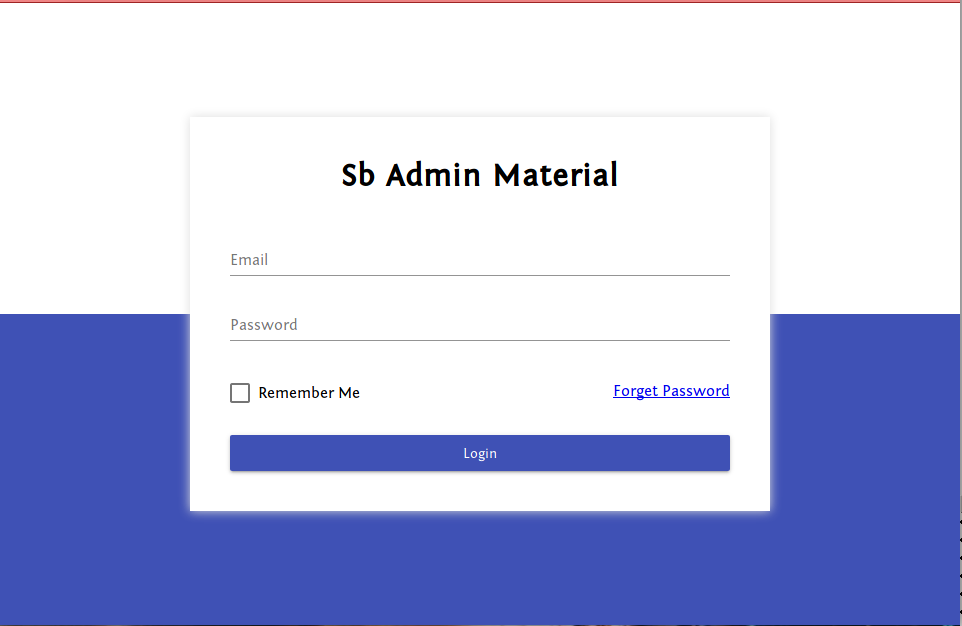
\includegraphics[width=.5\textwidth]{images/sbadmin/login}
  \caption{Login Screen}\label{fig:login}
\end{figure}
\begin{figure}
  \centering
  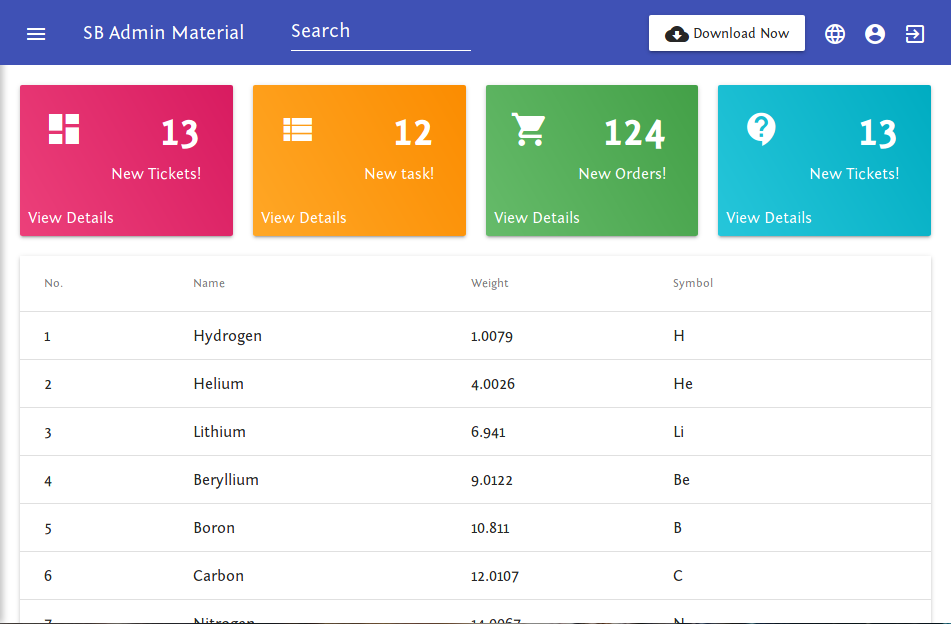
\includegraphics[width=.5\textwidth]{images/sbadmin/collapsed}
  \caption{Dashboard with collapsed side menu}\label{fig:dash}
\end{figure}
\begin{figure}
  \centering
  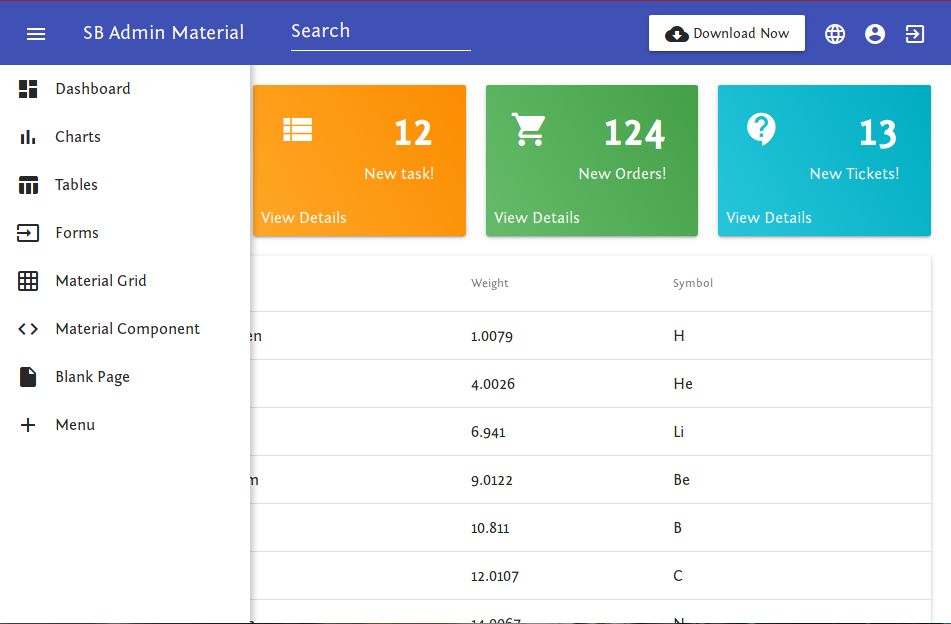
\includegraphics[width=.5\textwidth]{images/sbadmin/visible}
  \caption{Dashboard with visible side menu}\label{fig:visible}
\end{figure}

\subsubsection{Project Structure}
% introduction
SB Admin Angular was written with the intention of being modified and extended by other developers. Because the team did not express any guidelines towards how it should be further developed, it is important to give an overview of the current project structure so that the changes made to accommodate the topic of this project are better understood.

\begin{itemize}
\item \textbf{root} This item is not a folder but the root of the project. In here there are configurations for code linter, JavaScript dependency descriptor and the license statement.
\item \textbf{dist} Once the project is built for deployment, this directory will hold all the assets and optimized code ready for production, including the main \texttt{index.html} file that bootstraps the whole project.
\item \textbf{e2e} This holds the source code for End-to-End test cases, hence the name.
\item \textbf{src} This is the heart of this template, a directory that holds all the structure, content and behavior needed per application. \leavevmode
  \begin{itemize}
  \item \textbf{app} The Angular entry-point and application wide router module. \leavevmode
    \begin{itemize}
    \item \textbf{layout} All the components used to compose the navigational elements and menus and their subsequent pages plus some example pages. \leavevmode
      \begin{itemize}
      \item \textbf{black-page} A inaccessible component that does nothing, probably unfinished.
      \item \textbf{blank-page} An example component that is white.
      \item \textbf{charts} A component that display chart capabilities of the integrated JavaScript module chartjs\footnote{Available at https://www.chartjs.org/}.
          \item \textbf{components} Omnipresent page elements such as the Topbar and the collapsible Sidebar.\leavevmode
        \begin{itemize}
        \item \textbf{topnav} The blue navigation top bar as seen on Figure \ref{fig:dash}.
        \item \textbf{sidebar} The Menu on the left side of the screen as seen on Figure \ref{fig:visible}.
        \end{itemize}
      \item \textbf{dashboard} The page in which the user is redirected after logging in.
      \item \textbf{forms} Demonstration of the many different input methods such as Auto Complete text input, Date picker, Text Area and others.
      \item \textbf{grid} A demo of the available page subdivisions.
      \item \textbf{material-components} An example page displaying the main components of Angular Material such as buttons, Dialog and Notifications.
      \item \textbf{nav} Unused component, deprecated by the side bar component.
      \item \textbf{tables} A example component displaying Angular Material's table mechanisms.
      \end{itemize}

    \item \textbf{login} This is the Login component as see on Figure \ref{fig:login}
    \item \textbf{shared} Code that can be used in a application wide manner so that higher abstractions and code reuse can be achieved.
    \end{itemize}
  \item \textbf{assets} Static content directory. Images, fonts, and i18n translations.
  \item \textbf{environments} Depending on how the project is run, either in development or in production mode, a the respective configuration file that holds environment constants is used, allowing developers to use the same reference name throughout the code base no matter the environment.
  \item \textbf{styles} \gls{SASS} files that define the look and feel.
  \end{itemize}
\end{itemize}

% connection
After this overview, it is interesting to note the following:
\begin{itemize}
\item The Layout folder hosts, for the most part, Components and Modules that are listed in the sidebar.\item There are some unused components that were probably left over from design changes and were not deleted, which is the case of black-page and the nav component.
\item There are many examples that proved as a handy reference during development, namely the forms and material-components.
\end{itemize}

\section{Back-end}\label{cha:concepts:sec:backend}
The tools and concepts described in this section refer to the server-side of this project. It manages the authenticated and authorized data access as well as business-specific functionalities.

\subsection{Java}
% introduction
Given how ubiquitous it is, there is not much to be said. Java is a Object-Oriented programming language firstly developed by James Gosling at Sun Microsystems, it is statically and explicitly typed and gets compiled to a machine-independent byte code that is then interpreted by the \gls{JVM}~\cite{java}.

Because of its high adoption, many concepts were developed to accommodate its deficiencies and improve the development cycle. In fact, because of the recurring solutions for recurring situations in software design, a group of skilled professionals got together to discuss and write a book entitled ``Design Patterns: Elements of Reusable Object-Oriented Software''~\cite{patterns}, bringing the concept of repeatable ways to some problem.

% connection
This leads to the next topic, View Model, which was used throughout the development of this project to filter the information that is sent to a non-administrator user, removing from the role of filtering sensitive information to the insecure front-end application.

\subsubsection{View Model}
The ViewModel is a piece of a bigger pattern called \gls{MVVM} created by John Gossman to address the scenario in which a model as described in the \gls{MVC} pattern can't be completely mapped to a View~\cite{viewmodel}, therefore it is sensible to specify another model that partially reflects the original model but is able to be completely bound to user interface elements.

During the implementation of this project, the ViewModel pattern was used out of the \gls{MVVM} pattern, however the goal of decoupling code the same. More precisely, some models can not have all of its attributes serialized back to a View or they expose different attributes depending on the user who is requesting it; ViewModel classes were implemented in such cases.

\subsection{Spring}
% introduction
Developed by Pivotal Software in 2002, the Spring Framework provides most of the ``plumbing'' necessary for fast development and deployment of enterprise Java applications~\cite{springdocs}, some of the main features include: Dependency Injection, a \gls{IoC} mechanism; Spring Data, a set of tools for information access such as \gls{ORM} configurations; Spring Security, a application-wide security mechanisms and configurations.

One of the strongest design philosophies of the Spring Framework is the following:
\begin{displayquote}
``Provide choice at every level. Spring lets you defer design decisions as late as possible. For example, you can switch persistence providers through configuration without changing your code. The same is true for many other infrastructure concerns and integration with third-party \gls{API}s.''~\cite{springdocs}
\end{displayquote}
This leads to a feature-centered development model that is able to quickly deliver prototypes and changes on-demand.

\subsubsection{Dependency Injection}
Conceptually, Dependency Injection is a implementation of the \gls{IoC} principle, abdicating any given class class from managing its own dependencies; leaving them to a overseer object that knows how to create and inject dependencies to each class\cite{inversion}.

In practical terms, when writing a new class the programmer declare its dependencies through some mechanism in which the framework is able to reason about. Later in the run-time when a such dependent class is about to be instantiated, its dependencies are made available and injected into the new instance.

The key idea is that for the most part an application does not need to know which specific class is provided as long as it implements some given interface. It is the Framework's job to choose which class is injected. The programmer, however, is able to tailor the Framework's behavior to their liking.

When using Spring, one can express dependencies by declaring them in the class's constructor or by annotating an attribute using the Autowired annotation\cite{springdi}.

\subsubsection{Data}
When developing a enterprise-level application, often times there is the need of a database management system, an authentication provider and other information-centered services. To address this heterogeneous information storages the Spring Data module was developed that bases itself in a single interface named Repository, through which data is accessed\cite{springdata}.

For the general case the following modules cover the requirements of many applications:
\begin{itemize}
\item Spring Data \gls{JDBC}.
\item Spring Data \gls{JPA}.
\item Spring Data \gls{LDAP}.
\item Spring Data \gls{REST}
\end{itemize}
Note that these libraries are included with the bigger, Spring Data Project.

\subsubsection{\gls{HATEOAS}}
\gls{REST}, according to its creator:

\begin{displayquote}
  ``REST is a coordinated set of architectural constraints that attempts to minimize latency and network communication, while at the same time maximizing the independence and scalability of component implementations. This is achieved  by  placing  constraints  on  connector  semantics,  where  other  styles have focused on component semantics. REST enables the caching and reuse of interactions, dynamic substitutability of components, and processing of actions by intermediaries, in order to meet the needs of an Internet-scale distributed hypermedia system.''~\cite{fielding}
\end{displayquote}

In other words, this ``new'' architecture expresses requests and responses as the application state itself being transmitted in the client and server approach. There are a few ways in which the state can be communicated and structured, one of which is the subject of this section. 

\gls{HATEOAS} is a response structure that enables a client to discover and navigate related information for that resource\cite{fielding}. Mainly it is able to specify what are the related information, where it is located and how to interact with it. This is accomplished by including some meta-data in the response in which the client can parse, present to the user and issue proper requests.

In the context of Spring Framework, \texttt{CrudRepository} is a interface which can be extended for each class with Entity annotation that needs integration with some kind of persistence mechanism. In its default implementation there is a \gls{REST} service that is coherent with \gls{HATEOAS}, providing \gls{CRUD} capabilities; indexing as in listing all entries and internal resource linking, which give the ability to retrieve a resource's related resource (think of if like a \gls{RDBMS} table relation).

\subsubsection{Security}
This spring project aims to provide both authentication and authorization mechanisms throughout the application's components, exposing implementable interfaces that enable developers to override necessary parts for their specific needs.

It is important to clarify the distinction between Authentication and Authorization because they have their respective software counterpart that play important roles in Spring Framework.

Authentication, in by definition means ``To prove real or genuine''~\cite{merriamwebster}. In Spring this translates to a custom extension of the \texttt{WebSecurityConfigurerAdapter} abstract class that defines how to verify that a given user exists and is allowed access the resources. There are a few ways to achieve this, two of the most common are: \gls{JDBC} authentication, though which credentials are queried and matched from a \gls{RDBMS} and \gls{LDAP} authentication, that binds to some remote directory for the given user and password pair. Note that it does not define \textit{what} may be accessed by such user, only if the used has access to the system as a whole.

Authorization, ``the act of endorsing, or permitting by some recognized authority''~\cite{merriamwebster}. Similarly to Authentication can also be specified via a custom extension of \texttt{WebSecurityConfigurerAdapter}, and they can co-exist in the same extension. Authorization mechanisms are usually related to some attribute of the current authenticated user, in Spring, the \texttt{GrantedAuthority} interface is the central piece that unifies \textit{what} the user has access to. Authorization points can be defined at the global level by the \texttt{WebSecurityConfigurerAdapter}, at the controller level or at the method level though proper annotations.

\subsubsection{Boot}
Although Spring Framework is a marvelous piece of software for its malleability and wide range of available features, for a while it was considered a \textit{Configuration Hell} because of its \gls{XML} configuration that would require a lot of expertise into writing~\cite{xmlhell1}~\cite{xmlhell2}~\cite{xmlhell3}~\cite{xmlhell4}~\cite{xmlhell5}. In face of this, the Spring Team came up with Spring Boot, a dependency that can be inserted into a project and provides sane, already-configured Spring packages to accelerate development and keep code organized.

\subsection{MariaDB}
Due to legal concerns Michael Monty Widenius founded Monty Program AB, whose main product, MariaDB, started as a fork of his previous work, the MySQL \gls{RDBMS}~\cite{MAVRO:2014}. Such relational databases allow the user to define data structures and perform operations such as inserts, retrievals, updates and removals through a language known as \gls{SQL}

MariaDB is an open source project licensed under the \gls{GPL} and its current stable version is 5.2. Its \gls{SQL} dialect is and configuration files are either identical or very similar to those of MySQL. One of the main goals of MariaDB is to keep enhancing its performance~\cite{BARTHOLOMEW:2012}

MariaDB server is said to properly execute in many operating systems, namely Microsoft Windows, Solaris, Linux, MacOS and Free BSD. There are many packages that handle connections to MariaDB, graphically like DBeaver or phpMyAdmin, textually like mycli and not further than that, programming language connectors such as Java's \gls{JDBC}~\cite{MARIADB:2019}.

\subsection{Apache Directory Studio}\label{ads}
\gls{LDAP} in its core is a protocol defined by \gls{IETF}'s \gls{RFC} number 4511~\cite{ldaprfc} that defines access to X.500 compliant directory services. A Directory is an agglomerations of cooperative systems that serve structured information about the real world~\cite{x500}. Different from a traditional \gls{RDBMS}, directory services are expected to be automatically accessed by other interconnected systems, therefore they are better optimized for frequent queries and fewer updates.

Alex Karasulu, founder of the Apache Directory Project, was right when he stated that the need for interconnected systems grew alongside the expansion of the Internet but unlike his expectation, Directory services were replaced with \gls{RDBMS} systems that don't exactly address the same goals and further complicate interconnected systems\cite{apachedp}.

Given this situation, his project have the goal to modernize the tooling and functionalities of Directory systems and in doing so, two main sub-projects were created: Apache Directory Service~\cite{apachedservice}, a modern, \gls{LDAP}v3 compatible, Java based implementation of a Directory Service that introduces triggers, stored procedures, view and queues; Apache Directory Studio~\cite{apacheds}, a complete \gls{LDAP} tool developed as an Eclipse \gls{RCP} extension that offers a more friendly user experience with visual elements for  \gls{LDIF} editor, tree explorer and permission management.

\section{Development}\label{development}
This section cover the tools used during the development phase of this project. The tools in question do not only satisfy the coding needs but also mimics the production environment through which the application interacts with so that no sensitive information was touched by a potentially insecure, unfinished application.

In general, there was a need to comfortably edit Java and Angular projects, with code completion and refactoring support; a project manager that automatically downloads dependencies; a container tool to quickly deploy an environment with databases and directory services, without the need of editing non-functional configurations and lastly, a browser to access the system as the end-user would.

\subsection{Apache NetBeans}\label{netbeans}
One of the Duke's Choice Award winner~\cite{dukechoice}, NetBeans is a general-purpose, cross-platform \gls{IDE} mainly focused for Java development with the goal to maximize productivity. In 2016 NetBeans was added to the Apache Incubator so that it could be further developed by the community~\cite{incubation}, as of 2019 it became one of Apache's Top Level project~\cite{graduation} and is expected to attract a even bigger community.

Because Java was the main focus of NetBeans during its first few years, support for the language is very broad in features. Developers can easily operate code with context-sensitive refactoring; mark line, method, expression and class breakpoints; step through paused code; automatic JavaDoc generation; semantic code completion and more~\cite{nbassistance}.

Through its module system, support for other languages and resources were introduced, namely source code management with Git, Mercurial and Subversion, database management with support for viewing data and running \gls{SQL} queries, unit testing, PHP, HTML, JavaScript and CSS~\cite{nettutorials}.

\subsection{Maven}
Maven is a Build System for mainly used for Java applications, that is: Through a the \texttt{pom.xml} file, developers declare their project's attributes and dependencies file and if needed, tweak the building process; from there on, Maven is capable of downloading dependencies from a remote repository, compiling them if necessary and generate an executable \gls{JAR} file or loadable library~\cite{maven}.

The project goal is to unify the project structure so that there is less time spent by the developer to understand how the a given application code is arranged and to centralize common project actions such as previouly mentioned dependency resolution, run unit and integration tests and generate packages that are able to be distributed~\cite{mavenintro}.

\subsection{Lombok}
This plugin offers an annotation-based code-scaffolding tool for class definitions. Give the right annotations, common methods like getters, setters and no attribute constructor are automatically generated in build or compile-time~\cite{lombok}. This tool consists of a two-part system that includes the integration with the compiler/build-system and another one that interacts with the developer's \gls{IDE} so that the completion system is able to recognize the implicitly generated methods.

Some of the notable annotations include:
\begin{itemize}
\item \texttt{@Data}, useful for \gls{POJO} classes, this annotation generates getters, setters, a string converter and equality methods.
\item \texttt{@NoArgsConstructor} and \texttt{@AllArgsConstructor}, as the name implies, one generates a constructor that takes no arguments and the other, a constructor that generates all arguments.
\end{itemize}

At first glance this might not be a necessary tool given that most \gls{IDE}s often have support for a similar form of code refactoring but the key difference is that lombok does not clutter the classes with generated implementation therefore it reduces the project's \gls{LoC} count.

\subsection{Visual Studio Code}
Microsoft's take on open-source, this code editor gained traction among developers as one of the most used code editors~\cite{vscodesurvey}. Like any other modern code editor, it offers syntax highlight; auto-completion, though Microsoft's \textit{IntelliSense} integration and a plugin system that enables users to add custom behavior and further develop the editor's support for programming languages~\cite{vscode}.

One of the acclaimed features that arose with Visual Studio Code was the open source specification of \gls{LSP}~\cite{lsplaunch}. This specification aims to define a communication protocol that is used between a code editor, referred as a \gls{LSP} client and a editor-independent program referred as a \gls{LSP} server, that takes care of features such as code completion, highlight, error detection, contextual variable renaming and jumping to definition~\cite{lspspec}. This decoupling reduces the amount of code needed to develop a highly capable editor because language-dependent support is now transferred to said \gls{LSP} server.

\subsection{Docker}
Akin to a \gls{VM}, containers provides a way to have a different computing environment than the active running in the hardware. The key difference is that instead of emulating the whole computing stack, from processor to applicaion, a container system shares the core host resources with its guests and thus is generally less resource-hungry. One downside of a container is that the guest operating system must share the same kernel with the host.

In the other hand, Docker is more than just the sandboxing of processes, handling image building through a \texttt{Dockerfile} specification, containers that can be shared among different machines, a online registry of extendable containers, a command line interface that downloads, builds and manages containers~\cite{dockerfag}.

Core Docker definitions are brought up~\cite{dockeroverview}:
\begin{description}
\item[Dockerfile] A file that declares the steps taken to build an Image~\cite{dockerfile}.
\item[Image] A blueprint of a container generated once a \texttt{Dockerfile} is built.
\item[Container] If an image is an compiled binary, a container is the running process. 
\item[Volume] Is a shared folder between the host \gls{OS} and a running container.
\end{description}

\subsection{Docker-compose}
The flexibility offered by the Docker ecosystem is of great use for moderate applications. Define a \texttt{Dockerfile}, build it into an image and create a running container. However, not all solutions require a single image, in fact, most of them are composed of independently working pieces that are tailored together and bundling all pieces in a single image is not considered good practice~\cite{dockerfag}.

Distributed with Docker, this tool provides a way to define a multi-container applications, their virtual connections and manage all containers as one single entity. Such separation of concerns enable the tool to take smarter choices when starting a solution that includes a modified image, preserving volume data between solution runs and on the development side, it makes a local instance of a solution to be quickly deployed to testing purposes~\cite{compose}. 

\subsection{Chinook Database}
This is a single-script data-set. Structured in many \gls{SQL} dialects, it represents a  digital media store and in total it contains 11 tables, 11 constraints, 66 columns and 15607 rows~\cite{schemaspy}. The data used for this project was generated from a real iTunes library, sales information was randomly generated and customer and employee were manually inserted~\cite{chinook}.

List of Available dialects:
\begin{itemize}
\item MySQL
\item SQL Server
\item SQL Server Compact
\item SQLite
\item PostgreSQL
\item Oracle
\item DB2
\end{itemize}

Such diversity in dialects, structural complexity and amount of information makes the Chinook Database a good sample for database-generic applications.

\subsection{Angular CLI}\label{angularcli}
Angular applications have a basic directory for its components. Often times a directory contains most of the code for a specific piece of an application, such as a Component definition, a Service, a Template, a Style definition, a Class definition and lastly, these related pieces are then declared in a Module definition.

Managing this volume of files and relations can sometimes lead to confusion. Angular \gls{CLI} was developed to make this task more manageable. With it a developer can quickly initialize a new application skeleton, generate Components and Modules, build a deployment-ready applicaion and run a testing server that re-compile with code changes~\cite{angularcli}.

\subsection{Firefox}
From the downfall of Netscape browser and the release of its source code, the Mozilla project started with the mission to ensure the Internet to be a global public place, open and accessible to all~\cite{firemission}. Its main product is the open source web browser, Firefox.

Firefox comes bundled with plenty of tools that facilitate web development, considered as the most valuable are the following:
\begin{description}
\item [Source Mapping] Is the ability to map some generated code back to its source. Some web frameworks like Angular\ref{concept:angular} generate applications that are not developed in JavaScript itself but compiled to JavaScript in order to be executed~\cite{srcmapping}. In the beginning this led to great confusion because the browser's built-in debugger would display not the original source but the generated code.
\item [Debugger] Support for breakpoints, conditional breakpoints, expression stepping and variable lookup. Even better with the previous element~\cite{dbgmodernweb}.
\item [Network Monitor] Often times it is needed to inspect the outgoing requests and their responses. The integrated monitor is able to expose all elements of the communication exchange and measure the different attributes of a network operations~\cite{networkmon}.
\item [Storage Inspector] Provides access to the information storage that is managed by the browser for each page~\cite{storageinspector}, namely:
  \begin{itemize}
  \item Cache Storage
  \item Cookies
  \item Indexed \gls{DB}
  \item Local Storage
  \item Session Storage
  \end{itemize}
\item [Console] Enables the input of expressions in the page context and output information associated to the current page, including explicit calls for the \texttt{console.log} function.
\item [Page Inspector] Examine the page's \gls{HTML} structure and \gls{CSS} rules~\cite{inspector}. Developers can quickly experiment new possibilities by temporarily altering \gls{CSS} rules and the page's structure.
\end{description}

\subsection{Webpack}
With the growing complexity of web applications, websites got slower and development, trickier. Webpack was developed to generate a optimized, ready to run, package that can be deployed in production~\cite{webpack}. Such packages are not meant for code only, they may contain images, \gls{CSS} rules and anything else. It offers an \gls{API} that can transform the contents of a package before it is bundled, for example, Typescript sources and its compiled counterpart or extracting inline \gls{CSS} from a \gls{HTML} document into a separate file.

In the context of Firefox's debugger and an angular 2+ applications, when serving the application using Angular \gls{CLI}, discussed in Section ~\ref{angularcli}, it automatically bundles Typescript source code so that it can be instrumented and debugged inside the browser by accessing the Webpack element under the debugging tab.

\subsection{Postman}
As programs grew larger and were split into smaller pieces, it is now a common practice to have a \gls{API} that concentrate on the business logic and a \gls{GUI}s that consume them; Such separation of concerns got even more pronounced when Web systems popularized, web browsers acting as \gls{GUI} and interacting with remote \gls{HTTP} servers as their source of information.

As with any software, \gls{API}s need to be tested and validated in order to provide a good quality product. In this context Postman was developed to be a Web \gls{API} suite, offering a nice user interface through which developers can not only send, receive and analyze \gls{HTTP} requests but also generate and manage documentation so that front-end and back-end teams have a single source of truth, manage test cases for remote \gls{HTTP} \gls{API}s, mock \gls{API} that are still under development and more~\cite{postman}.